\lstset{frame=single,
  basicstyle=\footnotesize ,
  backgroundcolor=\color{white},
  language=Python}

\section{Managing Workflows}

\label{chap:pw}

\subsection{Overview}

Figure~\ref{fig:overview} provides a graphical illustration of the
components of a workflow.  A \textit{workflow} is comprised of one or more
computational steps, which we call a \textit{task} or \textit{component}.
A task maps a set of input data into a set of output data.  Input and
output data are managed with \textit{port} objects, and tasks are linked
together with \textit{connectors} that define a connection from an output
port in one task to an input port for another.  These connections form
a directed acyclic graph (DAG), which defines how task executions need
to be coordinated to correctly execute the entire workflow.

\begin{figure}[htb]
  \center
  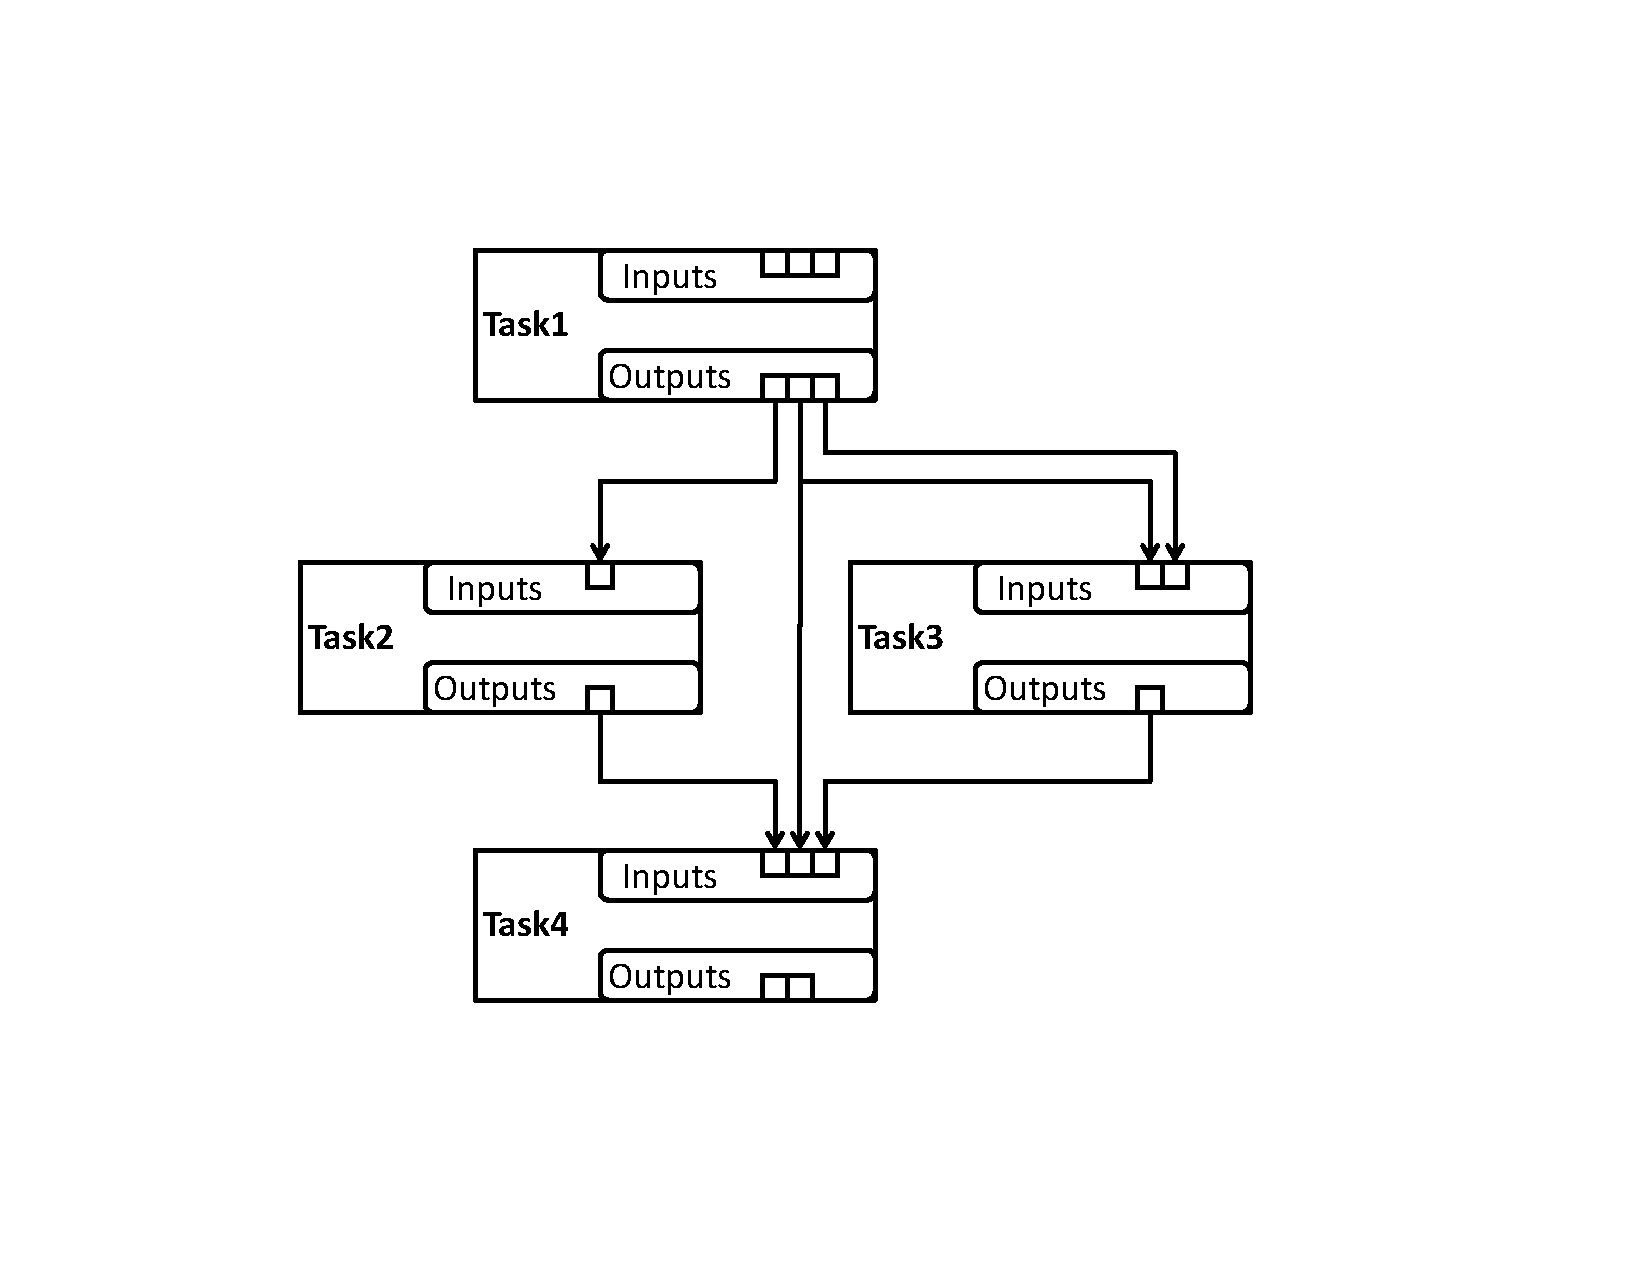
\includegraphics[height=5in]{figures/workflow-overview.pdf}
  %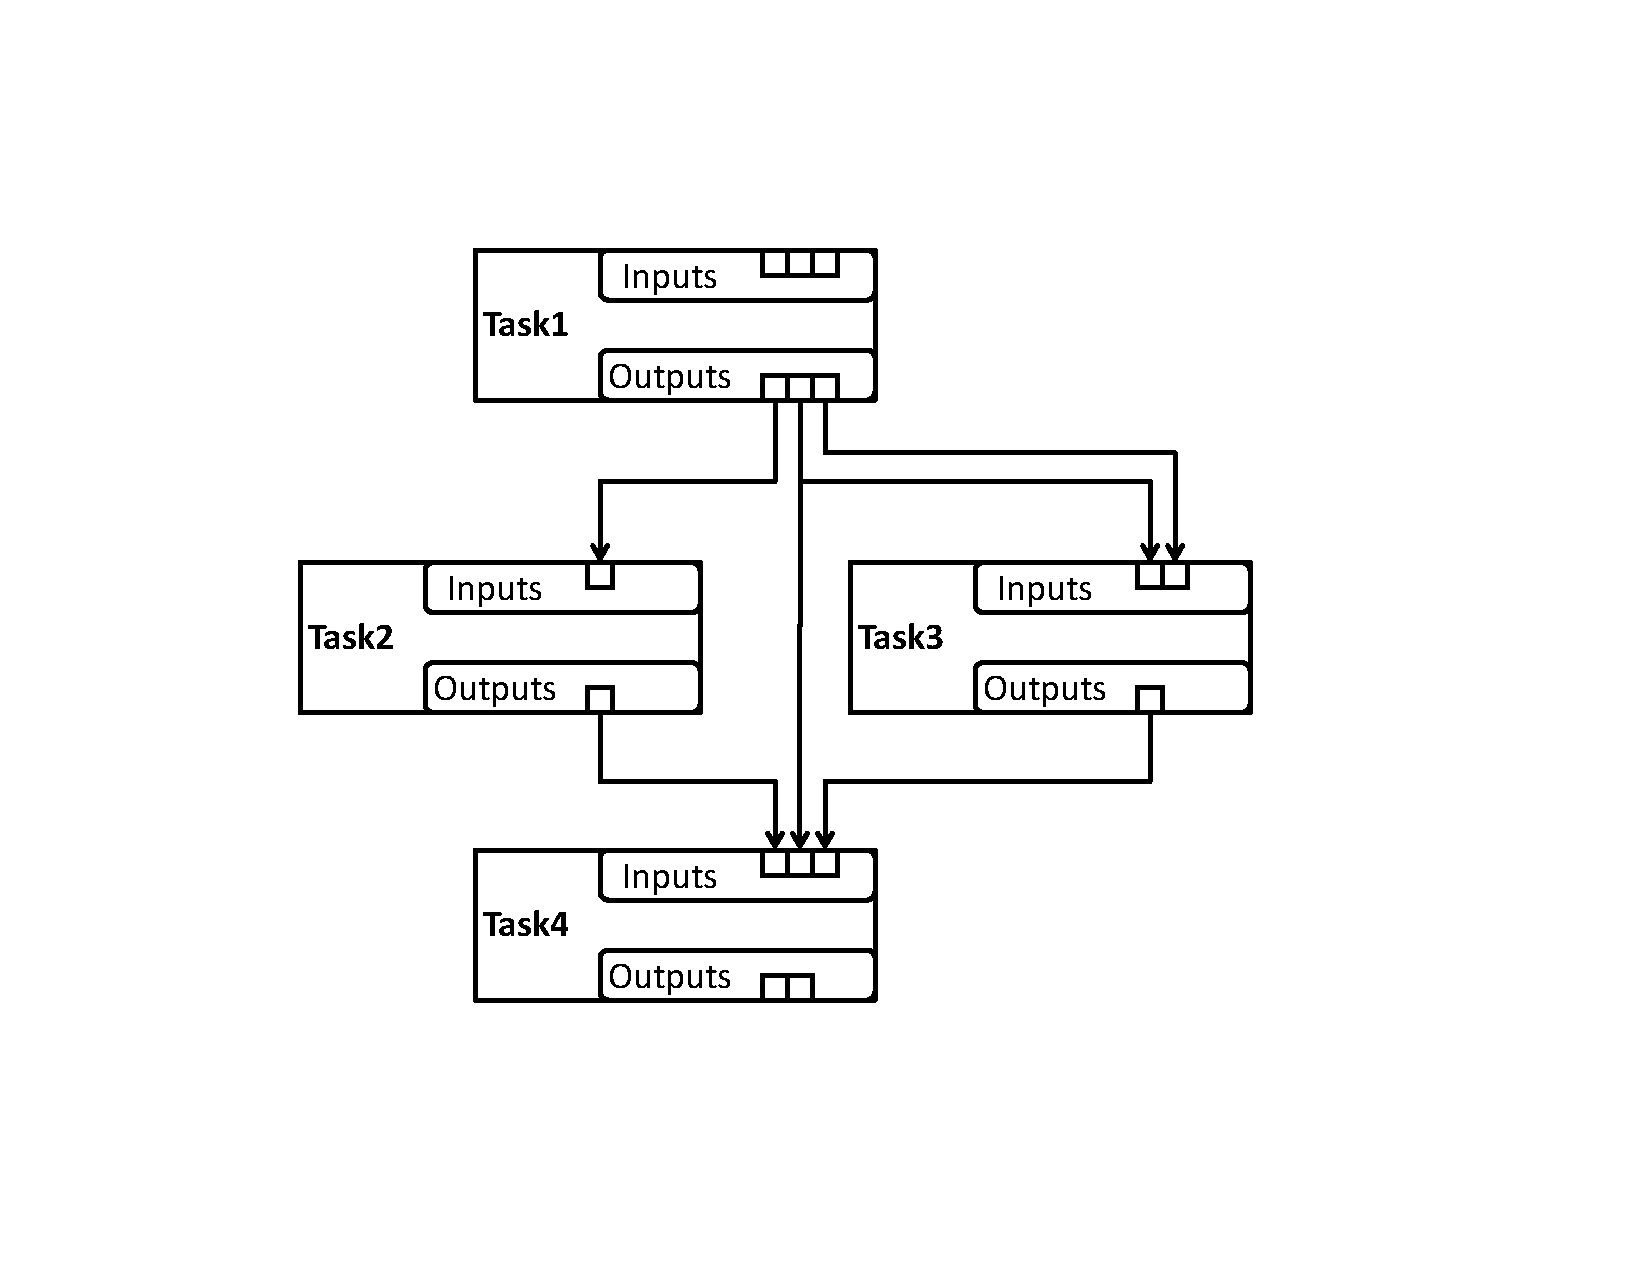
\includegraphics[height=5in,angle=-90]{figures/workflow-overview.pdf}
  \caption{A graphical illustration of a workflow with four tasks.  Black lines
between tasks represent connectors, and square boxes in the tasks represent the
input and output ports.}
  \label{fig:overview}
\end{figure}


\subsection{A Simple Example}
\label{sec:simple}

The main goal of \pwsp is to support the definition of workflows in an
intuitive manner using Python objects.  There are two fundamental classes defined
by \pwsp that are used to define a workflow: \code{Task} and \code{Workflow}.  
A user defines tasks by creating subclasses of the \code{Task} class.  For example,
the following task computes the sum of its two inputs:
\listing{examples/example1.py}{class}{4}{15}

The \code{Task} class defines the \code{inputs} and \code{outputs}
attributes that are used to respectively declare input and output ports.
These declarations must be included in the task constructor, since the
inputs and outputs are treated as static task properties by \pw.

The task computation is performed by the \code{execute} method, which
must be defined by the user.  Note that the input and output values are
attributes of the task object.  This simplifies the syntax for users
developing task computations by allowing them to treat task data as they
would in any other Python object.  \pwsp initializes the value of these
attributes before calling \code{execute}, and it interrogates the task
afterwards to set the value of the output ports.

The following Python code creates the \code{TaskA} object, creates a \code{Workflow}
object, initializes the workflow with this task, and then executes the workflow
with input values:
\listing{examples/example1.py}{usage}{18}{21}
Note that the workflow defines a functor, which is executed with keyword arguments that are mapped to the task inputs.  This functor returns an \code{Options} object, which is a glorified Python dict class.  The output of printing the workflow results is:
\listing{examples/example1.txt}{}{1}{1}



\subsection{Defining Connections}

The previous example was a trivial illustration of the setup and execution of a workflow.  In practice, workflows will be defined by constructing two or more tasks that are linked together.  Suppose we wish to compute the expression:
\[
z = 2*x+y.
\]
We can employ \code{TaskA} to perform the sum, and the following task to double the value of $x$:
\listing{examples/example2.py}{class}{17}{27}

The following Python code creates the \code{TaskA} and \code{TaskB} objects, links the output of B to the input of A, and then creates and executes a workflow:
\listing{examples/example2.py}{usage}{31}{37}
The connection between \code{TaskA} and \code{TaskB} is defined with the command
\begin{qlisting}
A.inputs.x = B.outputs.Z
\end{qlisting}
The syntax transparently creates a \code{Connector} object that connects the \code{Z} output of \code{TaskB} to the \code{x} input of \code{TaskA}.  This greatly simplifies
the declaration of connections when compared with other Python workflow packages.  Note that this mechanism allows an output port to be connected to one or more
input ports.  The default setup of ports allows an input port to only connect to a single output port.  (See Section~\ref{sec:multi-input} for further discussion.)

As in our earlier example, the workflow is created by constructing a \code{Workflow} object and then adding tasks to it.  Note, however, that in this example only \code{TaskA} was added.  The \code{Workflow} object traverses the connections between tasks to identify all tasks connected to the task that is added.  Consequently, 
only a single task in a workflow needs to be added to the \code{Workflow} object.

Note that the functor defined by the workflow has a slightly different API
in this example;  it uses inputs \code{X} and \code{y}.  To understand
why, consider Figure~\ref{fig:example2}, which shows the workflow
in this example.  Tasks \code{TaskA} and \code{TaskB} are connected
to each other, but also to a start and end task.  The start and end
tasks are constructed when a \code{Workflow} object loads the workflow.
The start task contains outputs that correspond to every input port that
is not connected to an output port.  Similarly, the end task contains inputs that 
correspond to every output port that is not connect to an input port.  In this way, the inputs and outputs of the workflow are automatically defined.

\begin{figure}[htb]
  \center
  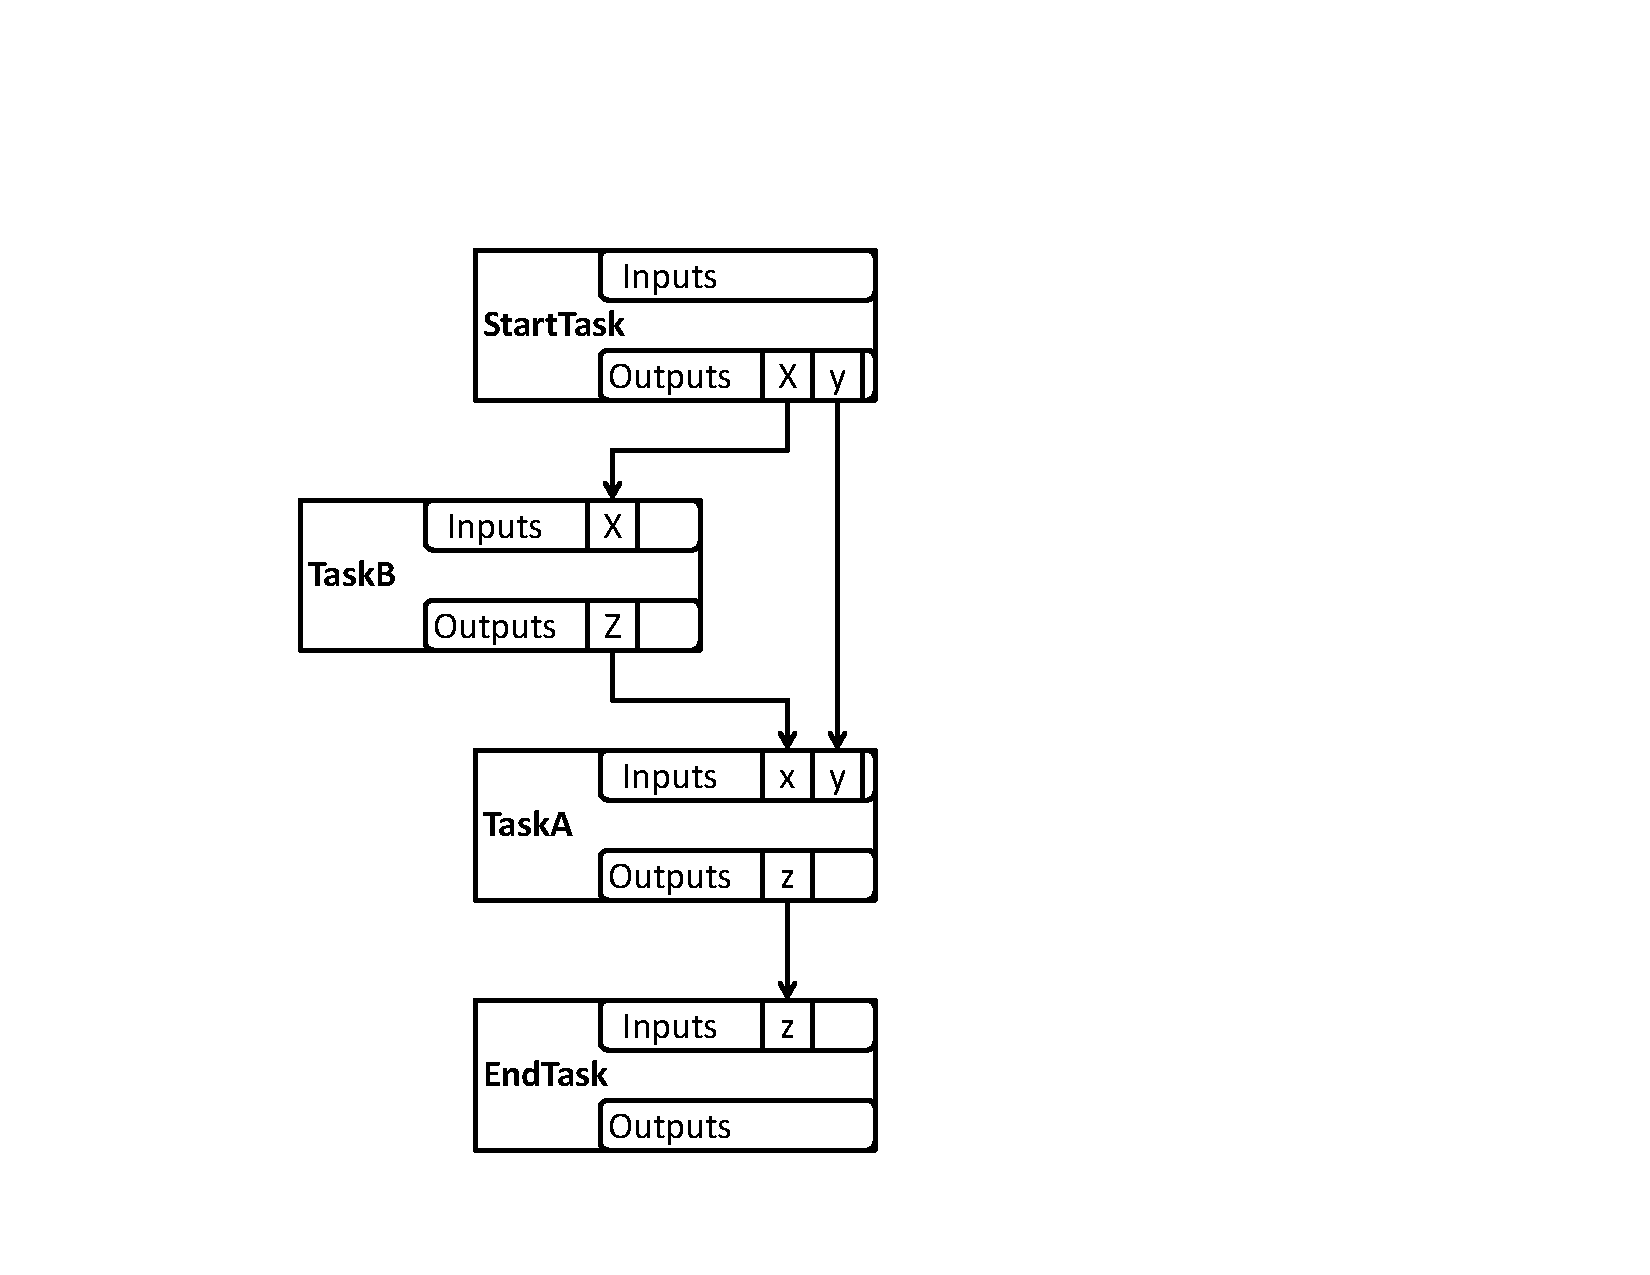
\includegraphics[height=5in]{figures/workflow-example2.pdf}
  %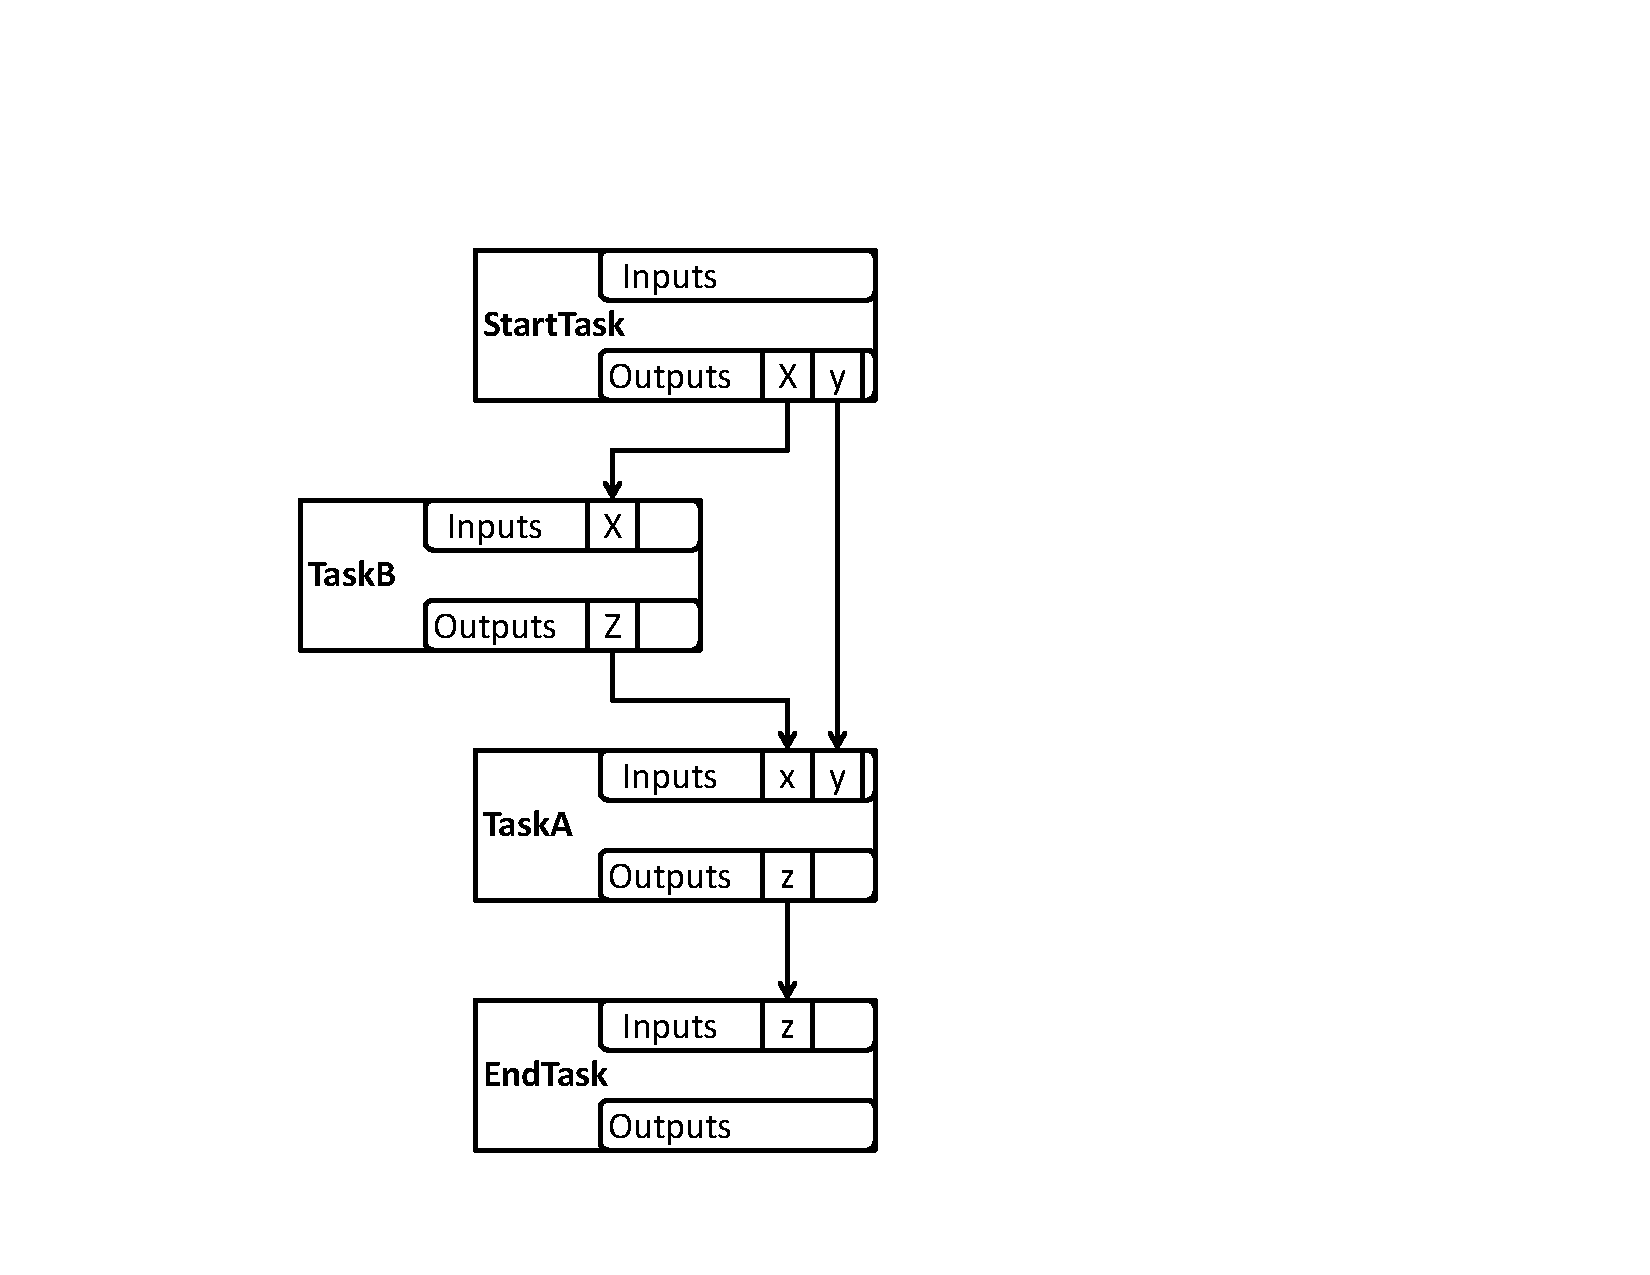
\includegraphics[height=5in,angle=-90]{figures/workflow-example2.pdf}
  \caption{An illustration of the workflow defined with tasks \code{TaskA} and \code{TaskB}.}
  \label{fig:example2}
\end{figure}

\begin{figure}[htb]
  \center
  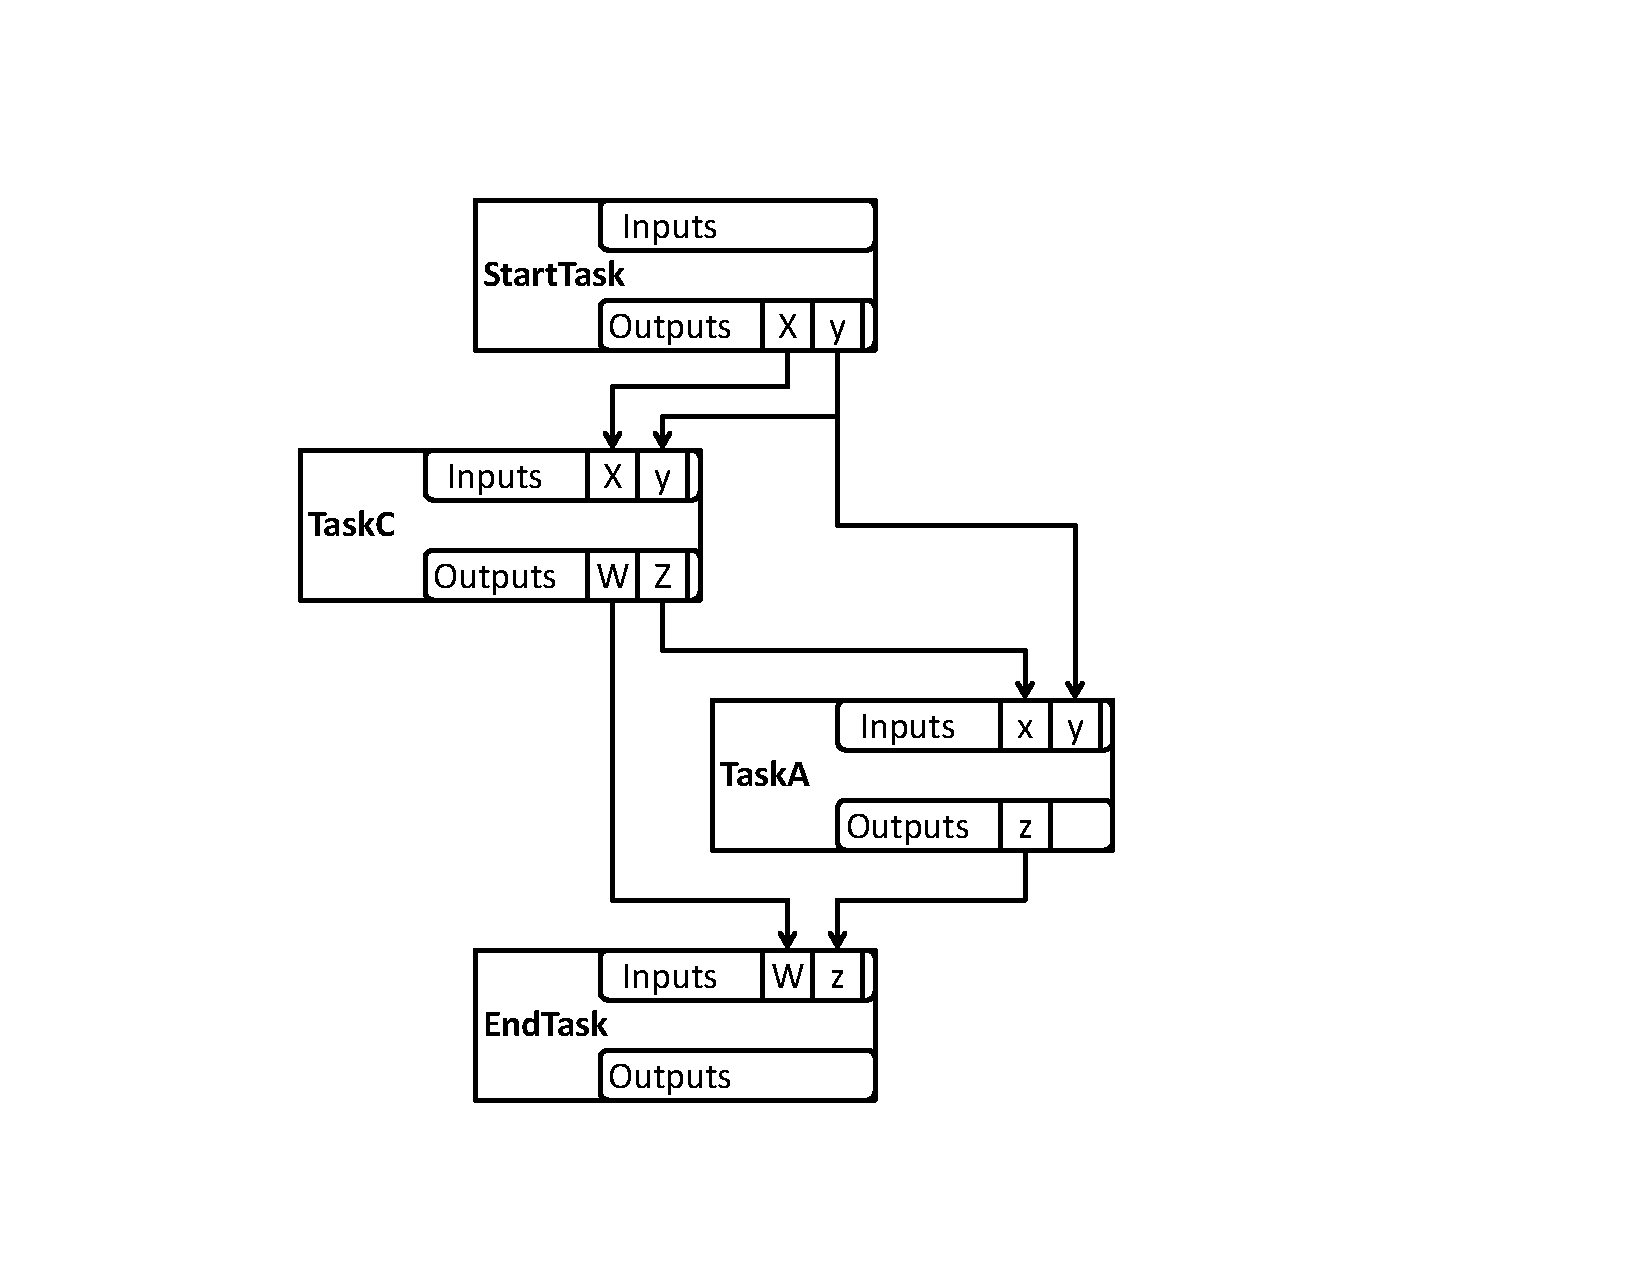
\includegraphics[height=5in]{figures/workflow-example3.pdf}
  %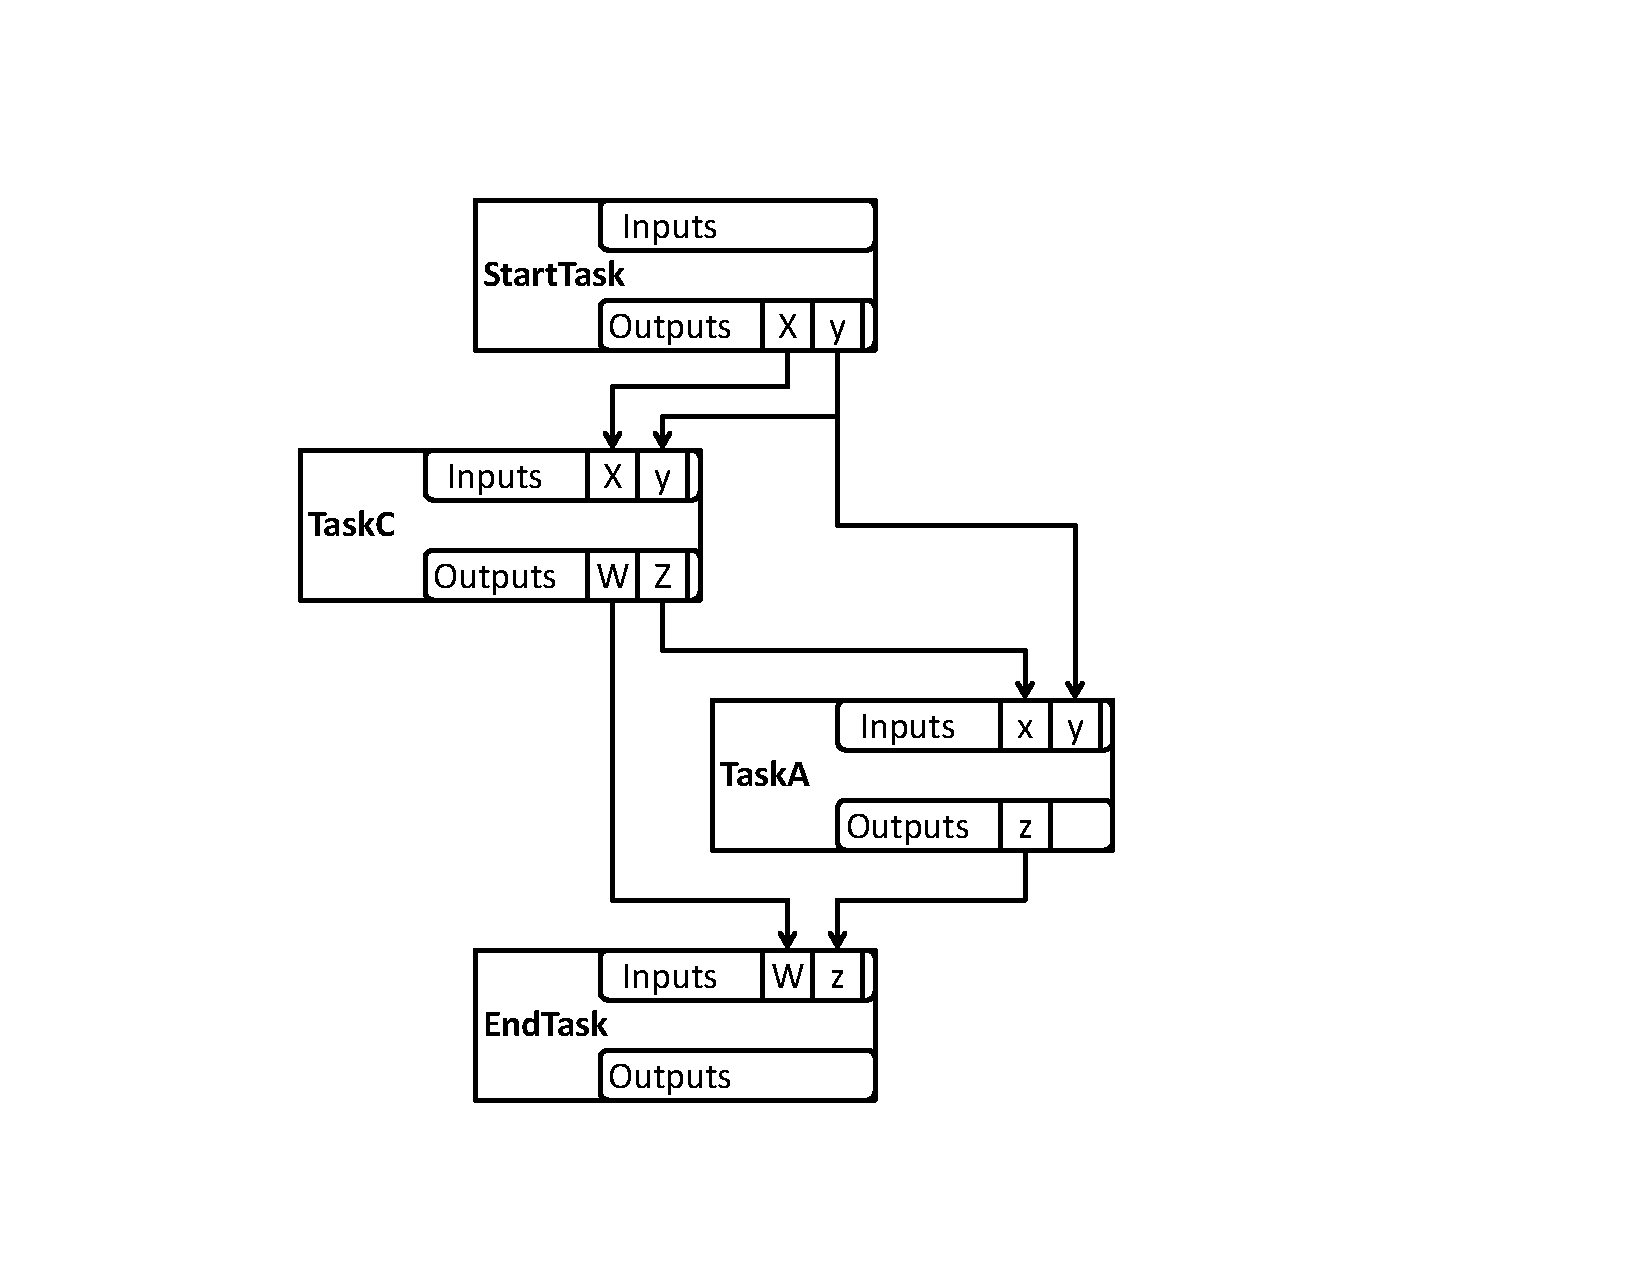
\includegraphics[height=5in,angle=-90]{figures/workflow-example3.pdf}
  \caption{An illustration of the workflow defined with tasks \code{TaskA} and \code{TaskC}.}
  \label{fig:example3}
\end{figure}

To see further implications of this logic, suppose that \code{TaskC} is used instead of \code{TaskB}:
\listing{examples/example3.py}{class}{17}{30}
Figure~\ref{fig:example3} shows the workflow for this example.  The setup and
execution of this task does not change.  However, the input \code{y} is now
used by both tasks \code{TaskA} and \code{TaskC}.  Further, the output \code{W}
is now included in the final results.  The output of printing the workflow results
is:
\listing{examples/example3.txt}{}{1}{2}
Similarly, the following example uses \code{TaskD} instead of \code{TaskB}:
\listing{examples/example3a.py}{class}{17}{31}
The input \code{a} is a constant
value that is not included in the outputs of the start task.  However, this value
can be set directly using the \code{TaskD} object.
The output of printing the workflow results
is:
\listing{examples/example3a.txt}{}{1}{2}


\subsection{Input Ports with Multiple Connections}

\label{sec:multi-input}

The \code{action} constructor option for the \code{Port} class
defines how input connections are used to compute the input value.
The default action is \code{store}, which indicates that the connector
value is stored in the port.  This behavior reflects the previous
examples, and it is well-suited for workflows where there is a
direct correspondence between output ports and input ports.

However, contexts often arise in practice where a suite of tasks
needs to be computed and their results are analyzed together.  For
example, consider \code{TaskD} which generalizes \code{TaskA} to
sum an arbitrary number of inputs:
\listing{examples/example5.py}{class}{5}{15}
Note that the input port \code{x} is defined with the \code{append}
action, which configures it to create a list of input values.

The following example use \code{TaskD} to define a workflow with
inputs from \code{TaskE}, which generates a random integer value:
\listing{examples/example5.py}{usage}{19}{46}
In this example, \code{TaskE} objects are created and connected to
the \code{TaskD} object with the command:
\begin{qlisting}
D.inputs.x = E.outputs.Z
\end{qlisting}
The input \code{x} port is configured to append inputs to a list,
and no special syntax is needed to indicate how the connections are
configured between the \code{x} port and the \code{Z} ports.

The \code{map} action can also be specified to define an input as
a dictionary with keys that are the task ids from the connection
that generated the values.  For example, this can be used to associate
data generated in different branches of a workflow.  The following
example uses this associate to define a dictionary, which is the
final result:
\listing{examples/example6.py}{ex}{4}{55}
Tasks \code{TaskF1} and \code{TaskF2} simply map their inputs to
outputs.  Their outputs are connected to two inputs in \code{TaskG},
and these inputs are used to create a dictionary.  The output of
this computation is:
\listing{examples/example6.log}{}{1}{2}

Normally, an input port with the \code{store}, \code{append} or
\code{map} action cannot be evaluated if any of the output ports
connected to it is not in the \code{ready} state.  However, the
\code{store\_any}, \code{append\_any} and \code{map\_any} actions allow
any or all of the inputs to be in a non-ready state.  When the \code{store\_any} action 
is specified, the value is simply taken from the first connection that is in the
\code{ready} state.  When the \code{map\_any} action is specified, then a dictionary is formed
from all connections that are in the \code{ready} state.  Similarly, the \code{append\_any} action
appends all values from connections inthe \code{ready} state.


\subsection{Using Workflows as Tasks}

A key feature of \pwsp is the ability to use workflows as components of other workflows.  This is possible because \code{Workflow} is a subclass of \code{Task}.

For example, consider the following workflows that are defined with \code{TaskA} and
\code{TaskC}:
\listing{examples/example4.py}{ex}{32}{46}
Workflow \code{w1} is the workflow defined in the previous example.  This object is 
used to define workflow \code{w2}, which uses \code{TaskA} to sum the outputs of \code{w1}: \code{W} and \code{z}. The output of executing \code{w2} is
\listing{examples/example4.txt}{}{1}{1}


\subsection{Initializing Port Values}

Task ports are initialized through the execution of a workflow, and through the 
explicit specification of port values.  The simplest way to specify port values is to 
define them directly.  For example, consider the following variation of the
example in Section~\ref{sec:simple}:
\listing{examples/example1a.py}{ex}{17}{22}
The workflow is constructed as before, but the values of ports \code{x} and \code{y} are 
defined explicitly, and the execution of the workflow does not specify these values.

\pwsp also supports the initialization of port values with command-line options.
The goal of this capability is to facilitate the use of PyUtilib in
command-line applications, by allowing command-line options to be used
to directly initialize a workflow.
The following example is a simple extension of the example in Section~\ref{sec:simple}.
\listing{examples/example1b.py}{ex}{4}{23}
Some additional logic is added to the \code{TaskAA} class to specify the
command-line options.
In this example, the \code{set\_argument} method is used to initialize a
workflow with a list of option strings.  This syntax mimics the format of
data provided by \code{sys.argv}.  Again, the execution of the workflow
does not specify these values.

Note that port values specified in these ways are viewed as default values
for the port.  When a port value is computed from input connections,
then the port value will be overriden if the input connections provide
a non-trivial value.  For example, if the port action is \code{store},
then the value will be overriden if the input connection has a value
other than \code{None}.  Similarly, if the port action is \code{append}
or \code{map}, then the value will be overriden if one or more of the
input connections are not None.  

Additionally, port values are redefined by the workflow keyword options.
For example, in the following script we initialize input ports for \code{TaskAA}, which
are then redefined when the workflow is executed:
\listing{examples/example1c.py}{ex}{19}{23}
The output of this script is 
\listing{examples/example1c.txt}{}{1}{1}
which reflects the fact that the value of \code{y} was redefined by the workflow
keyword option.


\subsection{The Task Factory}

\pwsp leverages the PyUtilib Component Architecture~\cite{PCA} to support
the definition of a task factory.  The \pwsp task factory allows users
to create plugin tasks on the fly without requiring knowledge of where
these tasks are defined.  This capability exposes a variety of standard
tasks that are defined in \pwsp, and it can be used to create tasks that
are defined by third-party libraries in a standard manner.

The \code{TaskFactory} object defined in \pwsp is a functor.  This
functor can be used to create a task that has been registered as a
plugin.  For example, the \code{Selection\_Task} class is registered
with the string 'workflow.selection', and it can be instantiated
as follows:
\begin{qlisting}
task = pyutilib.workflow.TaskFactory('workflow.selection')
\end{qlisting}
Section~\ref{sec:predefined} describes the predefined tasks that are
provided with \pw.

A plugin task is created as a subclass of the \code{TaskPlugin}
class.  This registers this task as a plugin with the PyUtilib
Component Architecture.  The only additional step required for a
plugin task is to use the \code{alias} declaration to define the
string that is used to create this task in the task factory.

For example, the following code defines the task \code{PluginTaskA}
that is registered with the string 'TaskA':
\listing{examples/example_plugin.py}{class}{5}{18}
Note that the only difference with the definition of \code{TaskA}
is the specification of the base class and the \code{alias}
declaration.

The following Python code creates the \code{PluginTaskA} object,
creates a \code{Workflow} object, initializes the workflow with
this task, and then executes the workflow with input values:
\listing{examples/example_plugin.py}{usage}{22}{25}
This has the same logical steps as the example in Section~\ref{sec:simple}.
The only difference is that the task is created by the task factory.



\section{Control Flow Tasks}

The basic functionality provided by \pwsp can be characterized as
a data flow.  Each task represents a transformation of data in input
ports to data in output ports.  These tasks are networked together
in a data flow graph, in which tasks form a directed acyclic graph
where data flows from the start task(s) to the final task(s).

\pwsp extends this functionality by providing control flow logic.
Tasks include special ports, input and output control ports that
can be used to limit the execution of tasks.  An output control
port is connected to one or more input control ports.  If an output
control port is set to the \textit{ready} state, then the tasks
connected to this with an input control port can be executed.
Otherwise, these tasks are blocked until the output control port
changes state.

For example, the \code{Selection\_Task} class is a predefined task
whose inputs are a dictionary, \code{data}, and an indexing value,
\code{index}.  This task returns \code{selection}, which is simply
the value \code{data[index]}.  This task can be used to switch 
the execution based on the indexed value.  For example:
\listing{examples/example9a.py}{code}{4}{25}
This generates the following output:
\listing{examples/example9a.txt}{}{1}{2}

The \code{Switch\_Task} class is a predefined task that provides a similar 
functionality in this example.  However, rather than switching the data value, this class
switches the control flow for downstream tasks.  For example:
\listing{examples/example9b.py}{code}{4}{43}
This generates the following output:
\listing{examples/example9b.txt}{}{1}{4}

The \code{Branch\_Task} class provides a simpler version of the
same process executed by the \code{Switch\_Task} class.  This class
switches the control flow for two downstream tasks.  For example:
\listing{examples/example8.txt}{usage}{1}{1}
Here, the branches for \code{TaskA} and \code{TaskB} are specified
with a branch value that is a boolean.


\section{Defining Task Resources}

There are many contexts in which task execution is dependent on the
availability of external resources.  For example, data files may
need to be available, a database may need to be unlocked, or a
software license may need to be free.  \pwsp allows these constraints
on workflow execution to be represented with \code{Resource} objects
that represent the state of a dependent resource.  A resource may
or may not be available, and the workflow can lock and unlock a
resource as it employs it for execution.

\pwsp defines the \code{ExecutableResource}, which allows a user
to specify an executable that is automatically found by searching
the \code{PATH} environment.  If the specified executable is not
found, then it is unavailable for execution in a workflow.  This
resource also includes a utility method for applying this executable
with command-line arguments.

The following example illustrates the use of this resource to define
a task that lists all of the files in a specified directory:
\listing{examples/example7.py}{ex}{15}{36}

%Similarly, the \code{FileResource} allows a user to specify a file
%whose availability can affect the flow-control of a workflow.
%The following example illustrates the use of this 

A key role of resource objects is that they can limit the execution
of tasks.  The \code{availability} method in a resource object is
queried to see if a resource can be allocated.  The following example illustrates this
functionality with a simple \code{BusyResource} class that is busy the first time it is queried:
\listing{examples/example10.py}{ex}{1}{30}
The first time that task \code{A} is queried, this resource is not
available.  Note that the \pwsp workflow execution process currently does
not allow tasks to block indefinitely.  If all tasks have blocked, then the workflow execution will immediately terminate.  


\section{Predefined Tasks}
\label{sec:predefined}

The following sections describe the task plugins that are defined
by \pw, and we provide an example of how a task plugin is defined.

\subsection{Selection Task}

The \code{workflow.selection} task has the following inputs:
\begin{itemize}

\item \code{data}: a dictionary
\item \code{index}: an index key in the dictionary
\end{itemize}
This task returns the value of the dictionary with the specified index key.

Note that this task does not fail gracefully if the index key is not defined in the
dictionary.  An exception will occur that will terminate the execution of the 
workflow.


\section{The Task Driver}

The \pwsp task driver provides a facility for creating a command-line
utility that can execute \pwsp plugin tasks.  The task driver is inspired
by command-line tools like \code{svn} that allow users to specify
subcommands that have independent command-line arguments.
The \pwsp task driver can be easily configured to execute different
tasks and workflows as subcommands within a command-line application.

Consider the following two task classes:
\listing{examples/tasks_yz.py}{class}{5}{37}
Note that these are plugin tasks that can be created with the \code{TaskFactory} functor.  The \pwsp task
driver can only execute tasks and workflows that are defined as plugins.

Suppose that the 
\code{TaskZ} and \code{TasY} are defined in the file \code{task\_yz.py}.
The following script creates a task driver, activates two these two tasks and illustrates the results of
parsing two sets of command-line arguments:
\listing{examples/example_driver1.py}{usage}{5}{12}
However, the true value of the task driver is in the definition of a command-line utility.
For example, the following script defines a
command-line utility that can execute tasks \code{TaskZ} and \code{TaskY}:
\listing{examples/driver1.py}{}{1}{8}
This script creates the task driver and then parses the \code{sys.argv} command-line arguments.
Suppose that this script is in the file \code{driver1.py}.  Then the following command-line illustrates the
execution of task \code{TaskZ}:
\listing{examples/driver_1.sh}{code}{4}{4}
which generates the following output:
\listing{examples/driver_1.txt}{}{1}{1}

The task driver constructor includes several options for declaring the script name and associated
documentation that will be printed when the \code{--help} option is specified:
\begin{itemize}

\item {\bf prog} - The name of the script.

\item {\bf description} - A short description of the script's functionality.

\item {\bf epilog} - Additional documentation that is printed after the command-line options are described.
\end{itemize}
The following script uses these options to illustrate the help information that is printed by the task
driver:
\listing{examples/driver2.py}{}{1}{18}
Suppose that this script is in the file \code{driver2.py}.  Then the following command-line illustrates the
execution with the \code{--help} option:
\listing{examples/driver_3.sh}{code}{4}{4}
which generates the following output:
\listing{examples/driver_3.txt}{}{1}{20}
Furthermore, the \code{--help} option can be used to print information about a specific subcommand.  The 
command
\listing{examples/driver_2.sh}{code}{4}{4}
generates the following output:
\listing{examples/driver_2.txt}{}{1}{6}{}

